\section[Graph-based VND]{\thirdtitle}

\def\thirdtitleF{Graph representation of a solution space}
\def\thirdtitleS{Applying said graphs within a Variable Neighborhood Descent}

\begin{frame}
\frametitle{\textbf{Contents}}
  \setbeamercovered{transparent}
  \begin{block}{\textbf{\thirdtitleF}}
  \end{block}  

  \only<1>{
    \begin{block}{\textbf{\thirdtitleS}}
    \end{block}  
  }
  \only<2->{
    \transparent{0.3}
    \begin{block}{\textbf{\thirdtitleS}}
    \end{block}  
    \transparent{1}
  }

\end{frame}

\begin{frame}
\frametitle{\textbf{Patterns}}

  \DrawGantt{2}{2}{0}

\end{frame}

\begin{frame}
\frametitle{\textbf{Pattern representation}}
  \begin{adjustbox}{max totalsize={\textwidth}{\textheight},left, trim=15pt 0 0 0}
    \begin{tikzpicture}
	\begin{pgfonlayer}{nodelayer}
		\node [style=source] (0) at (-5, 0) {50/2};
		\node [style=blank] (2) at (-3, 0) {50/0};
		\node [style=blank] (8) at (-4, 0) {50/1};
		\node [style=maint] (13) at (-2, 2.75) {100/6};
		\node [style=maint] (14) at (-3, 2.75) {100/6};
		\node [style=maint] (17) at (4, 2.75) {100/6};
		\node [style=blank] (24) at (-1, 2.75) {100/5};
		\node [style=mission] (31) at (0, 0.75) {60/4};
		\node [style=sink] (32) at (5, 0) {*/*};
		\node [style=blank] (35) at (2, 0.75) {60/3};
		\node [style=blank] (36) at (0, 2.75) {100/4};
		\node [style=mission] (37) at (0, -0.5) {40/3};
		\node [style=blank] (38) at (3, -0.5) {40/2};
		\node [style=blank] (39) at (3, 0.75) {60/2};
		\node [style=blank] (42) at (4, -0.5) {40/1};
		\node [style=blank] (43) at (4, 0.75) {60/1};
		\node [style=blank] (44) at (1, 2.75) {100/3};
		\node [style=blank] (45) at (2, 2.75) {100/2};
		\node [style=blank] (46) at (3, 2.75) {100/1};
		\node [style=mission] (50) at (0, -1.5) {20/2};
		\node [style=blank] (51) at (4, -1.5) {20/1};
	\end{pgfonlayer}
	\begin{pgfonlayer}{edgelayer}
		\draw [style=arrow] (0) to (8);
		\draw [style=arrow] (8) to (2);
		\draw [style=arrow] (17) to (32);
		\draw [style=arrow] (24) to (36);
		\draw [style=arrow] (37) to (38);
		\draw [style=arrow] (35) to (39);
		\draw [style=arrow] (31) to (35);
		\draw [style=arrow] (38) to (42);
		\draw [style=arrow] (39) to (43);
		\draw [style=arrow] (43) to (32);
		\draw [style=arrow] (42) to (32);
		\draw [style=arrow] (36) to (44);
		\draw [style=arrow] (44) to (45);
		\draw [style=arrow] (45) to (46);
		\draw [style=arrow] (39) to (17);
		\draw [style=arrow] (38) to (17);
		\draw [style=arrow, in=-105, out=0, looseness=2.00] (50) to (17);
		\draw [style=arrow] (50) to (51);
		\draw [style=arrow] (51) to (32);
		\draw (46) to (17);
		\draw (2) to (13);
		\draw (8) to (14);
		\draw [bend left, looseness=1.25] (14) to (24);
		\draw [bend right=15, looseness=0.75] (24) to (31);
		\draw [bend right=15] (24) to (37);
		\draw [bend right=15] (24) to (50);
	\end{pgfonlayer}
\end{tikzpicture}

  \end{adjustbox}

  \only<1-3>{
  \DrawGantt{0}{0}{0}
  }
  \only<4-5>{
  \DrawGantt{1}{0}{0}
  }
  \only<6>{
  \DrawGantt{1}{2}{0}
  }
  \only<7->{
  \DrawGantt{2}{2}{1}
  }
  \begin{textblock*}{1.1\textwidth}(0.8cm, 8cm)
    \begin{flushleft}
    % $\star$
    \onslide<1>{
      \citesize $\star$ Q. Deng, B. F. Santos, and R. Curran. A practical dynamic programming based methodology for aircraft maintenance check scheduling optimization. European Journal of Operational Research, 2020.
    }
    \end{flushleft}
  \end{textblock*}
\end{frame}

\begin{frame}
\frametitle{\textbf{Pattern extraction}}
% \begin{tikzpicture}
  \only<1>{
  \DrawGantt{2}{2}{1}
  }
  \only<2-5>{
  \DrawGantt{2}{2}{milestones}
  }
  \only<6->{
  \DrawGantt{1}{3}{milestones}
  }
  % \onslide<2->{
  %   \ganttmilestone[milestone/.append style={anchor=west, fill=blue}]{}{4}
  %   \ganttmilestone[milestone/.append style={anchor=east, fill=blue}]{}{10}
  % }
% \end{tikzpicture}
  \onslide<3->{  
    \begin{adjustbox}{max totalsize={\textwidth}{\textheight},left, trim=15pt 0 0 0}
      \begin{tikzpicture}
% \setbeamercovered{transparent}
  \transparent{0.3}
    \node [style=blank] (0) at (-5, 0) {50/2};
    \node [style=blank] (8) at (-4, 0) {50/1};
    \draw [] (0) to (8);
    \node [style=maint] (14) at (-3, 2.75) {100/6};
    \node [style=blank] (2) at (-3, 0) {50/0};
    \draw (8) to (2);
    \node [style=maint] (13) at (-2, 2.75) {100/6};
    \draw (2) to (13);  
    \draw[] (8) to (14);
    \draw [bend left, looseness=1.25] (14) to (24);
  \transparent{1}

  \node [style=example] (exa) at (9.5, 3) {$rft$/$rct$};
   \node [style=source] (24) at (-1, 2.75) {100/5};
   \node [style=mission] (31) at (0, 0.75) {60/4};
  \node [style=blank] (36) at (0, 2.75) {100/4};
  \node [style=mission] (37) at (0, -0.5) {40/3};
  \node [style=mission] (50) at (0, -1.5) {20/2};
   \node [style=maint] (17) at (4, 2.75) {100/6};

  \only<2>{
    \node [style=blank] (51) at (4, -1.5) {20/1};
    \draw (50) to (51);
    \draw (51) to (32);
  }
   \node [style=sink] (32) at (5, 0) {*/*};

  \node [style=blank] (35) at (2, 0.75) {60/3};
  \node [style=blank] (38) at (3, -0.5) {40/2};
  \node [style=blank] (39) at (3, 0.75) {60/2};
  \node [style=blank] (42) at (4, -0.5) {40/1};
  \node [style=blank] (43) at (4, 0.75) {60/1};
  \node [style=blank] (44) at (1, 2.75) {100/3};
  \node [style=blank] (45) at (2, 2.75) {100/2};
  \node [style=blank] (46) at (3, 2.75) {100/1};

  \draw [bend right=15, looseness=0.75] (24) to (31);
  \draw [bend right=15] (24) to (37);
  \draw (24) to (36);
  \draw [bend right=15] (24) to (50);

  \draw [ in=-105, out=0, looseness=2.00] (50) to (17);
  \draw [] (17) to (32);
  \draw (37) to (38);
  \draw (35) to (39);
  \draw (31) to (35);
  \draw (38) to (42);
  \draw (39) to (43);
  \draw (43) to (32);
  \draw (42) to (32);
  \draw (36) to (44);
  \draw (44) to (45);
  \draw (45) to (46);
  \draw (39) to (17);
  \draw (38) to (17);
  \draw (46) to (17);

  \onslide<4>{
    \draw [bend right=15, looseness=0.75] (24) to node {$w_1$} (31);
    \draw [bend right=15] (24) to node {$w_2$} (37);
    \draw (24) to (36);
    \draw [bend right=15] (24) to node {$w_3$} (50);
    \draw [ in=-105, out=0, looseness=2.00] (50) to node {$w_4$} (17);
    \draw [] (17) to (32);
    \draw (37) to node {$w_6$} (38);
    \draw (35) to (39);
    \draw (31) to node {$w_5$} (35);
    \draw (38) to (42);
    \draw (39) to (43);
    \draw (43) to (32);
    \draw (42) to (32);
    \draw (36) to (44);
    \draw (44) to (45);
    \draw (45) to (46);
    \draw (39) to (17);
    \draw (38) to (17);
    \draw (46) to (17);
  }
  \onslide<5->{
    \draw [bend right=15, style=arrow] (24) to node {$w_2$} (37);
    \draw [style=arrow] (37) to node {$w_6$} (38);
    \draw [style=arrow] (38) to (42);
    \draw [style=arrow] (42) to (32);
  }

\end{tikzpicture}
    \end{adjustbox}
  }
\end{frame}

\begin{frame}
\frametitle{\textbf{Contents}}
  \setbeamercovered{transparent}
  \transparent{0.3}
  \begin{block}{\textbf{\thirdtitleF}}
  \end{block}  
  \transparent{1}

  \begin{block}{\textbf{\thirdtitleS}}
  \end{block}  
\end{frame}

\begin{frame}
\frametitle{\textbf{Solution approach: Variable Neighborhod Descent}}
  \pause
  \begin{adjustbox}{max totalsize={0.8\textwidth}{0.8\textheight},center}
  % \begin{tikzpicture}
          \begin{tikzpicture}
      [node distance=1.6cm,
      every node/.style={fill=white, font=\sffamily}, align=left]
     % Specification of nodes (position, etc.)
      \node (start)             [activityStarts]              {Start};

      % \onslide<+->{
        \node (initSol)     [startstop, below of=start]          {$x = getInitialSolution()$\\$z^* = \infty$\\$t = clock()$};
        \draw[->]             (start) -- (initSol);
      % }
      % \onslide<+->{
        \node (objFunc)      [master, below of=initSol]   {$err= getErrors(x)$\\$z=getObjective(x,err)$};
        \draw[->]     (initSol) -- (objFunc);
      % }
      % \onslide<+->{
         \node (maybeBest)      [master, below of=objFunc]   {$z < z^*$};
         \draw[->]     (objFunc) -- (maybeBest);
          \node (updateBest)      [master, right of=maybeBest, xshift=3cm]   {$x^* = x$\\$z^* = z$};
         \draw[->]      (maybeBest) -- node {Yes} (updateBest);
      % }
      % \onslide<+->{
        \node (maybeStop)      [master, below of=maybeBest, yshift=-0.5cm]   {$clock() -t > t_{max}$};
        \node (Stop)      [activityStarts, right of=maybeStop, xshift=3cm]   {End};
        \draw[->]     (maybeStop) -- node {Yes}  (Stop);
        \draw[->]      (maybeBest) -- node {No} (maybeStop);
        \draw[->]      (updateBest.south) -- ++(0,-.7) -- ++(-4.5,0)  -- (maybeStop.north);
      % }
      % \onslide<+->{
        \node (chooseNeighborFunc)     [master, below of=maybeStop, yshift=-0.5cm, neighborhoods]   {$move = choose\{S\hspace{-0.5mm}P\hspace{-0.5mm}A, RH\}$\\$\mathcal{T}_{c}, \mathcal{I}_{c} = getCandidate(err, move)$\\$x = move(x, \mathcal{T}_{c}, \mathcal{I}_{c})$};
        \draw[->] (chooseNeighborFunc.west) -- ++(-0.5,0) -- ++(0,3.8) -- ++(0,2) -- (objFunc.west);
        \draw[->]     (maybeStop) -- node {No} (chooseNeighborFunc);
      % }
 
      \end{tikzpicture}
  % \end{tikzpicture}
  \end{adjustbox}

\end{frame}

\begin{frame}
\frametitle{\textbf{Neighborhood 1: Shortest Path Algorithm (SPA)}}
  \onslide<2->{
    $SPA(x, \mathcal{I}_c, \mathcal{T}_c)$
  }

  \onslide<3->{
    \begin{align*}
      A_{c} = \left(
      \begin{array}{*6{c}}
    1 & 1 & 1 & 1 & 0 & 0 \\
    \tikzmarkM{left}{0} & {\text -}1 & {\text -}1 & {\text -}1 & {\text -}1 & \tikzmarkM{right}{0} \\
    0 & 0 & 0 & 0 & 2 & 2 \\
    0 & 0 & 0 & 0 & 0 & 0
      \end{array}
      \right)
      \Highlight[first]
    \end{align*}
  }
  \onslide<4->{
    \begin{align*}
      A_{c+1} = \left(
      \begin{array}{*6{c}}
    1 & 1 & 1 & 1 & 0 & 0 \\
    \tikzmarkM{left}{0} & 1 & 1 & 1 & 2 & \tikzmarkM{right}{-1} \\
    0 & 0 & 0 & 0 & 2 & 2 \\
    0 & 0 & 0 & 0 & 0 & 0
      \end{array}
      \right)
    \Highlight[second]
  \end{align*}
    \tikz[overlay,remember picture] {
      \draw[->,thick,red,dashed] (first.east) -- ++(2, -2)  node [right] {SPA} -- (second.east);
    }
  }

\end{frame}

\begin{frame}
\frametitle{\textbf{Neighborhood 2: Rolling Horizon (RH)}}
  
  \onslide<2->{
    $RH(x, \mathcal{I}_c, \mathcal{T}_c)$
  }
  \onslide<3->{
    \begin{align*}
      A_{c} = \left(
      \begin{array}{*6{c}}
        1 & \tikzmarkM{left}{1} & 1 & 1 & 0 & 0 \\
        {\text -}1 & 0 & 0 & 0 & 0 & {\text -}1 \\
        0 & 0 & 0 & \tikzmarkM{right}{0} & 2 & 2 \\
        0 & 0 & 0 & 0 & 0 & 0
      \end{array}
      \right)
      \Highlight[first]
    \end{align*}  
  }
  \onslide<4->{
    \begin{align*}
      A_{c+1} = \left(
      \begin{array}{*6{c}}
        1 & \tikzmarkM{left}{0} & 0 & 0 & 0 & 0 \\
        {\text -}1 & 0 & 0 & 0 & 0 & {\text -}1 \\
        0 & 1 & 1 & \tikzmarkM{right}{1} & 2 & 2 \\
        0 & 0 & 0 & 0 & 0 & 0
      \end{array}
      \right)
    \Highlight[second]
    \end{align*}
    \tikz[overlay,remember picture] {
      \draw[->,thick,red,dashed] (first.east) -- ++(4, -2) node [right] {RH} -- (second.east);
    }
  }
\end{frame}

\begin{frame}[t]
\frametitle{\textbf{Initial solution}}

  \begin{columns}[T]
    \column{0.5\linewidth}
    \begin{itemize}
      \onslide<1->{
        \item $SPA(\varnothing, \mathcal{I}, \mathcal{T})$
        \vspace{2.5cm}
      }
      \onslide<7->{       
        \item $RH(\varnothing, \mathcal{I}, \mathcal{T})$ 
        \vspace{2.5cm}
      }
      \onslide<9->{
        \item Simulated Annealing()
      }
    \end{itemize}

    \column{0.5\linewidth}
        \only<2>{
      \begin{align*}
        \left(
        \begin{array}{*6{c}}
          0 & 0 & 0 & 0 & 0 & 0 \\
          0 & 0 & 0 & 0 & 0 & 0 \\
          0 & 0 & 0 & 0 & 0 & 0 \\
          0 & 0 & 0 & 0 & 0 & 0
        \end{array}
        \right)
    \end{align*}
    }
    \only<3>{
      \begin{align*}
        \left(
        \begin{array}{*6{c}}
          0 & 0 & 0 & 0 & 0 & 0 \\
          \tikzmarkM{left}{0} & 1 & 1 & 1 & 2 & \tikzmarkM{right}{-1} \\
          0 & 0 & 0 & 0 & 0 & 0 \\
          0 & 0 & 0 & 0 & 0 & 0
        \end{array}
        \right)
      \Highlight[second]
    \end{align*}
    }
    \only<4>{
      \begin{align*}
        \left(
        \begin{array}{*6{c}}
          \tikzmarkM{left}{1} & 1 & 1 & 1 & 0 & \tikzmarkM{right}{0} \\
          0 & 1 & 1 & 1 & 2 & {\text -}1 \\
          0 & 0 & 0 & 0 & 0 & 0 \\
          0 & 0 & 0 & 0 & 0 & 0
        \end{array}
        \right)
      \Highlight[second]
    \end{align*}
    }
    \only<5>{
      \begin{align*}
       \left(
        \begin{array}{*6{c}}
          1 & 1 & 1 & 1 & 0 & 0 \\
          0 & 1 & 1 & 1 & 2 & {\text -}1 \\
          \tikzmarkM{left}{0} & 0 & 0 & 0 & 2 & \tikzmarkM{right}{2} \\
          0 & 0 & 0 & 0 & 0 & 0
        \end{array}
        \right)
      \Highlight[second]
    \end{align*}
    }
  \only<6>{
      \begin{align*}
        \left(
        \begin{array}{*6{c}}
          \tikzmarkM{left}{0} & 0 & 0 & 0 & 0 & 0 \\
          0 & 0 & 0 & 0 & 0 & 0 \\
          0 & 0 & 0 & 0 & 0 & 0 \\
          0 & 0 & 0 & 0 & 0 & \tikzmarkM{right}{0}
        \end{array}
        \right)
        \Highlight[first]
      \end{align*}
  }

    \only<7>{
      \begin{align*}
        \left(
        \begin{array}{*6{c}}
          \tikzmarkM{left}{1} & 1 & 1 & 1 & 0 & 0 \\
          0 & 1 & 1 & 1 & 2 & {\text -}1 \\
          0 & 0 & 0 & 0 & 2 & 2 \\
          0 & 0 & 0 & 0 & 0 & \tikzmarkM{right}{0}
        \end{array}
        \right)
      \Highlight[second]
    \end{align*}
    }

  \end{columns}

  % \begin{tabular}{ll}
  % \onslide<+->{
  %   $SPA(\varnothing, \mathcal{I}, \mathcal{T})$ &     \only<2>{
      \begin{align*}
        \left(
        \begin{array}{*6{c}}
          0 & 0 & 0 & 0 & 0 & 0 \\
          0 & 0 & 0 & 0 & 0 & 0 \\
          0 & 0 & 0 & 0 & 0 & 0 \\
          0 & 0 & 0 & 0 & 0 & 0
        \end{array}
        \right)
    \end{align*}
    }
    \only<3>{
      \begin{align*}
        \left(
        \begin{array}{*6{c}}
          0 & 0 & 0 & 0 & 0 & 0 \\
          \tikzmarkM{left}{0} & 1 & 1 & 1 & 2 & \tikzmarkM{right}{-1} \\
          0 & 0 & 0 & 0 & 0 & 0 \\
          0 & 0 & 0 & 0 & 0 & 0
        \end{array}
        \right)
      \Highlight[second]
    \end{align*}
    }
    \only<4>{
      \begin{align*}
        \left(
        \begin{array}{*6{c}}
          \tikzmarkM{left}{1} & 1 & 1 & 1 & 0 & \tikzmarkM{right}{0} \\
          0 & 1 & 1 & 1 & 2 & {\text -}1 \\
          0 & 0 & 0 & 0 & 0 & 0 \\
          0 & 0 & 0 & 0 & 0 & 0
        \end{array}
        \right)
      \Highlight[second]
    \end{align*}
    }
    \only<5>{
      \begin{align*}
       \left(
        \begin{array}{*6{c}}
          1 & 1 & 1 & 1 & 0 & 0 \\
          0 & 1 & 1 & 1 & 2 & {\text -}1 \\
          \tikzmarkM{left}{0} & 0 & 0 & 0 & 2 & \tikzmarkM{right}{2} \\
          0 & 0 & 0 & 0 & 0 & 0
        \end{array}
        \right)
      \Highlight[second]
    \end{align*}
    }
  \only<6>{
      \begin{align*}
        \left(
        \begin{array}{*6{c}}
          \tikzmarkM{left}{0} & 0 & 0 & 0 & 0 & 0 \\
          0 & 0 & 0 & 0 & 0 & 0 \\
          0 & 0 & 0 & 0 & 0 & 0 \\
          0 & 0 & 0 & 0 & 0 & \tikzmarkM{right}{0}
        \end{array}
        \right)
        \Highlight[first]
      \end{align*}
  }

    \only<7>{
      \begin{align*}
        \left(
        \begin{array}{*6{c}}
          \tikzmarkM{left}{1} & 1 & 1 & 1 & 0 & 0 \\
          0 & 1 & 1 & 1 & 2 & {\text -}1 \\
          0 & 0 & 0 & 0 & 2 & 2 \\
          0 & 0 & 0 & 0 & 0 & \tikzmarkM{right}{0}
        \end{array}
        \right)
      \Highlight[second]
    \end{align*}
    }

  %   } \\
  % \onslide<+->{
  %     $RH(\varnothing, \mathcal{I}, \mathcal{T})$  & 
  % } \\
  % % \onslide<+->{
  % %     \textbf{Input features} & $H(x) = \{h_m(x) \,\, \forall m \in \mathcal{M}\}$ 
  % % }\\ 
  % % \onslide<6->{
  % %     \textbf{Training for optimal} & $G(y^*(x)) \approx \hat{G}(x) = f(H(x)) \, \star$
  % % } \\
  % \end{tabular}

\end{frame}

\begin{frame}
\frametitle{\textbf{Experiments}}
  
  \begin{itemize}
    \item Instance sizes: large ($|I|$=60), very large ($|I|$=100) and \textbf{very} large ($|I|$=255).
    \item 1 graph per cluster of aircraft and node aggregation with respect to remaining flight time.
    \item CPLEX running 1 thread for up to 20 minutes.
  \end{itemize}
  All instances have 90 periods.
\end{frame}

\begin{frame}
\frametitle{\textbf{Results: comparing neighborhoods}}
  \begin{itemize}
    \item SPA: fast but reaches local minima.
    \item RH: slow but avoids local minima.
    \item VND=SPA+RH: fast and avoids local minima.
  \end{itemize}

  \begin{block}{}
    Example of one instance ($|I|$=60) solved 5 times with different random seeds, for 5 minutes.
    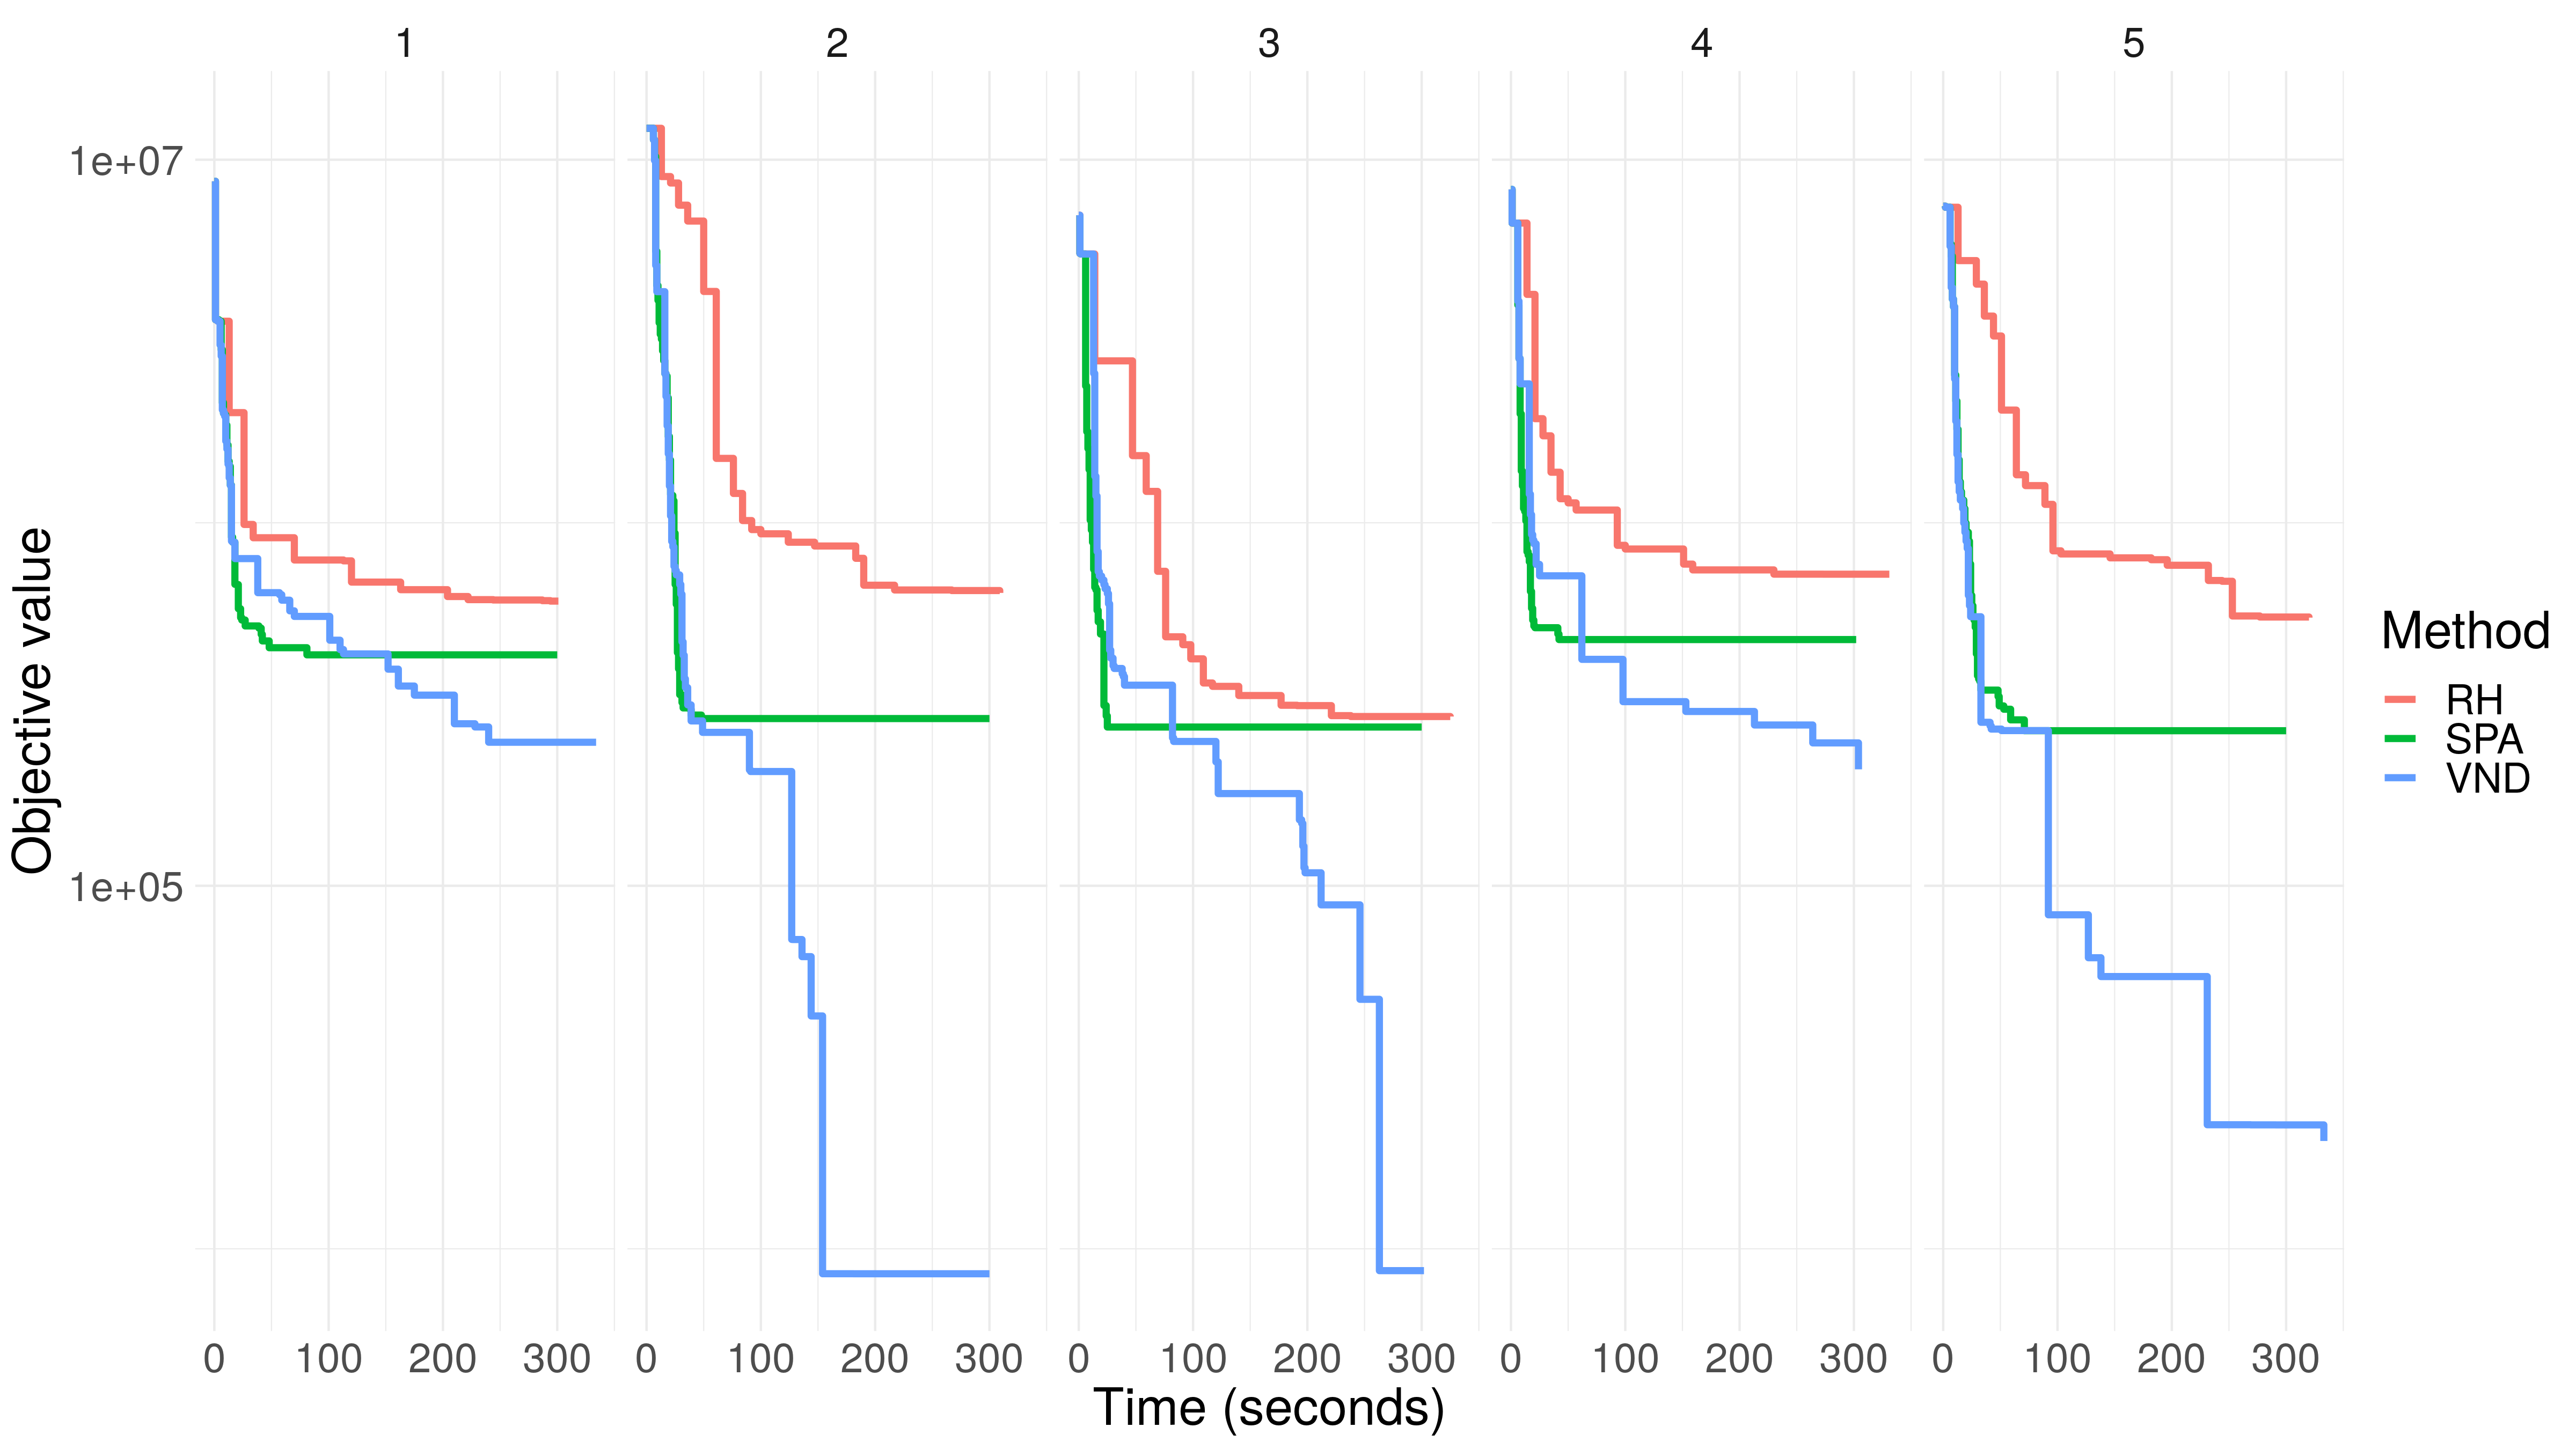
\includegraphics[width=0.8\linewidth]{images/compare_neighbors.png}
  \end{block}
\end{frame}

\begin{frame}
\frametitle{\textbf{Results: large instances}}
  \begin{itemize}
    \item VND outperforms MIP for very large instances (255 aircraft).
  \end{itemize}

  \begin{block}{}
    Example comparing the percentage gap to the best known lower bound.
    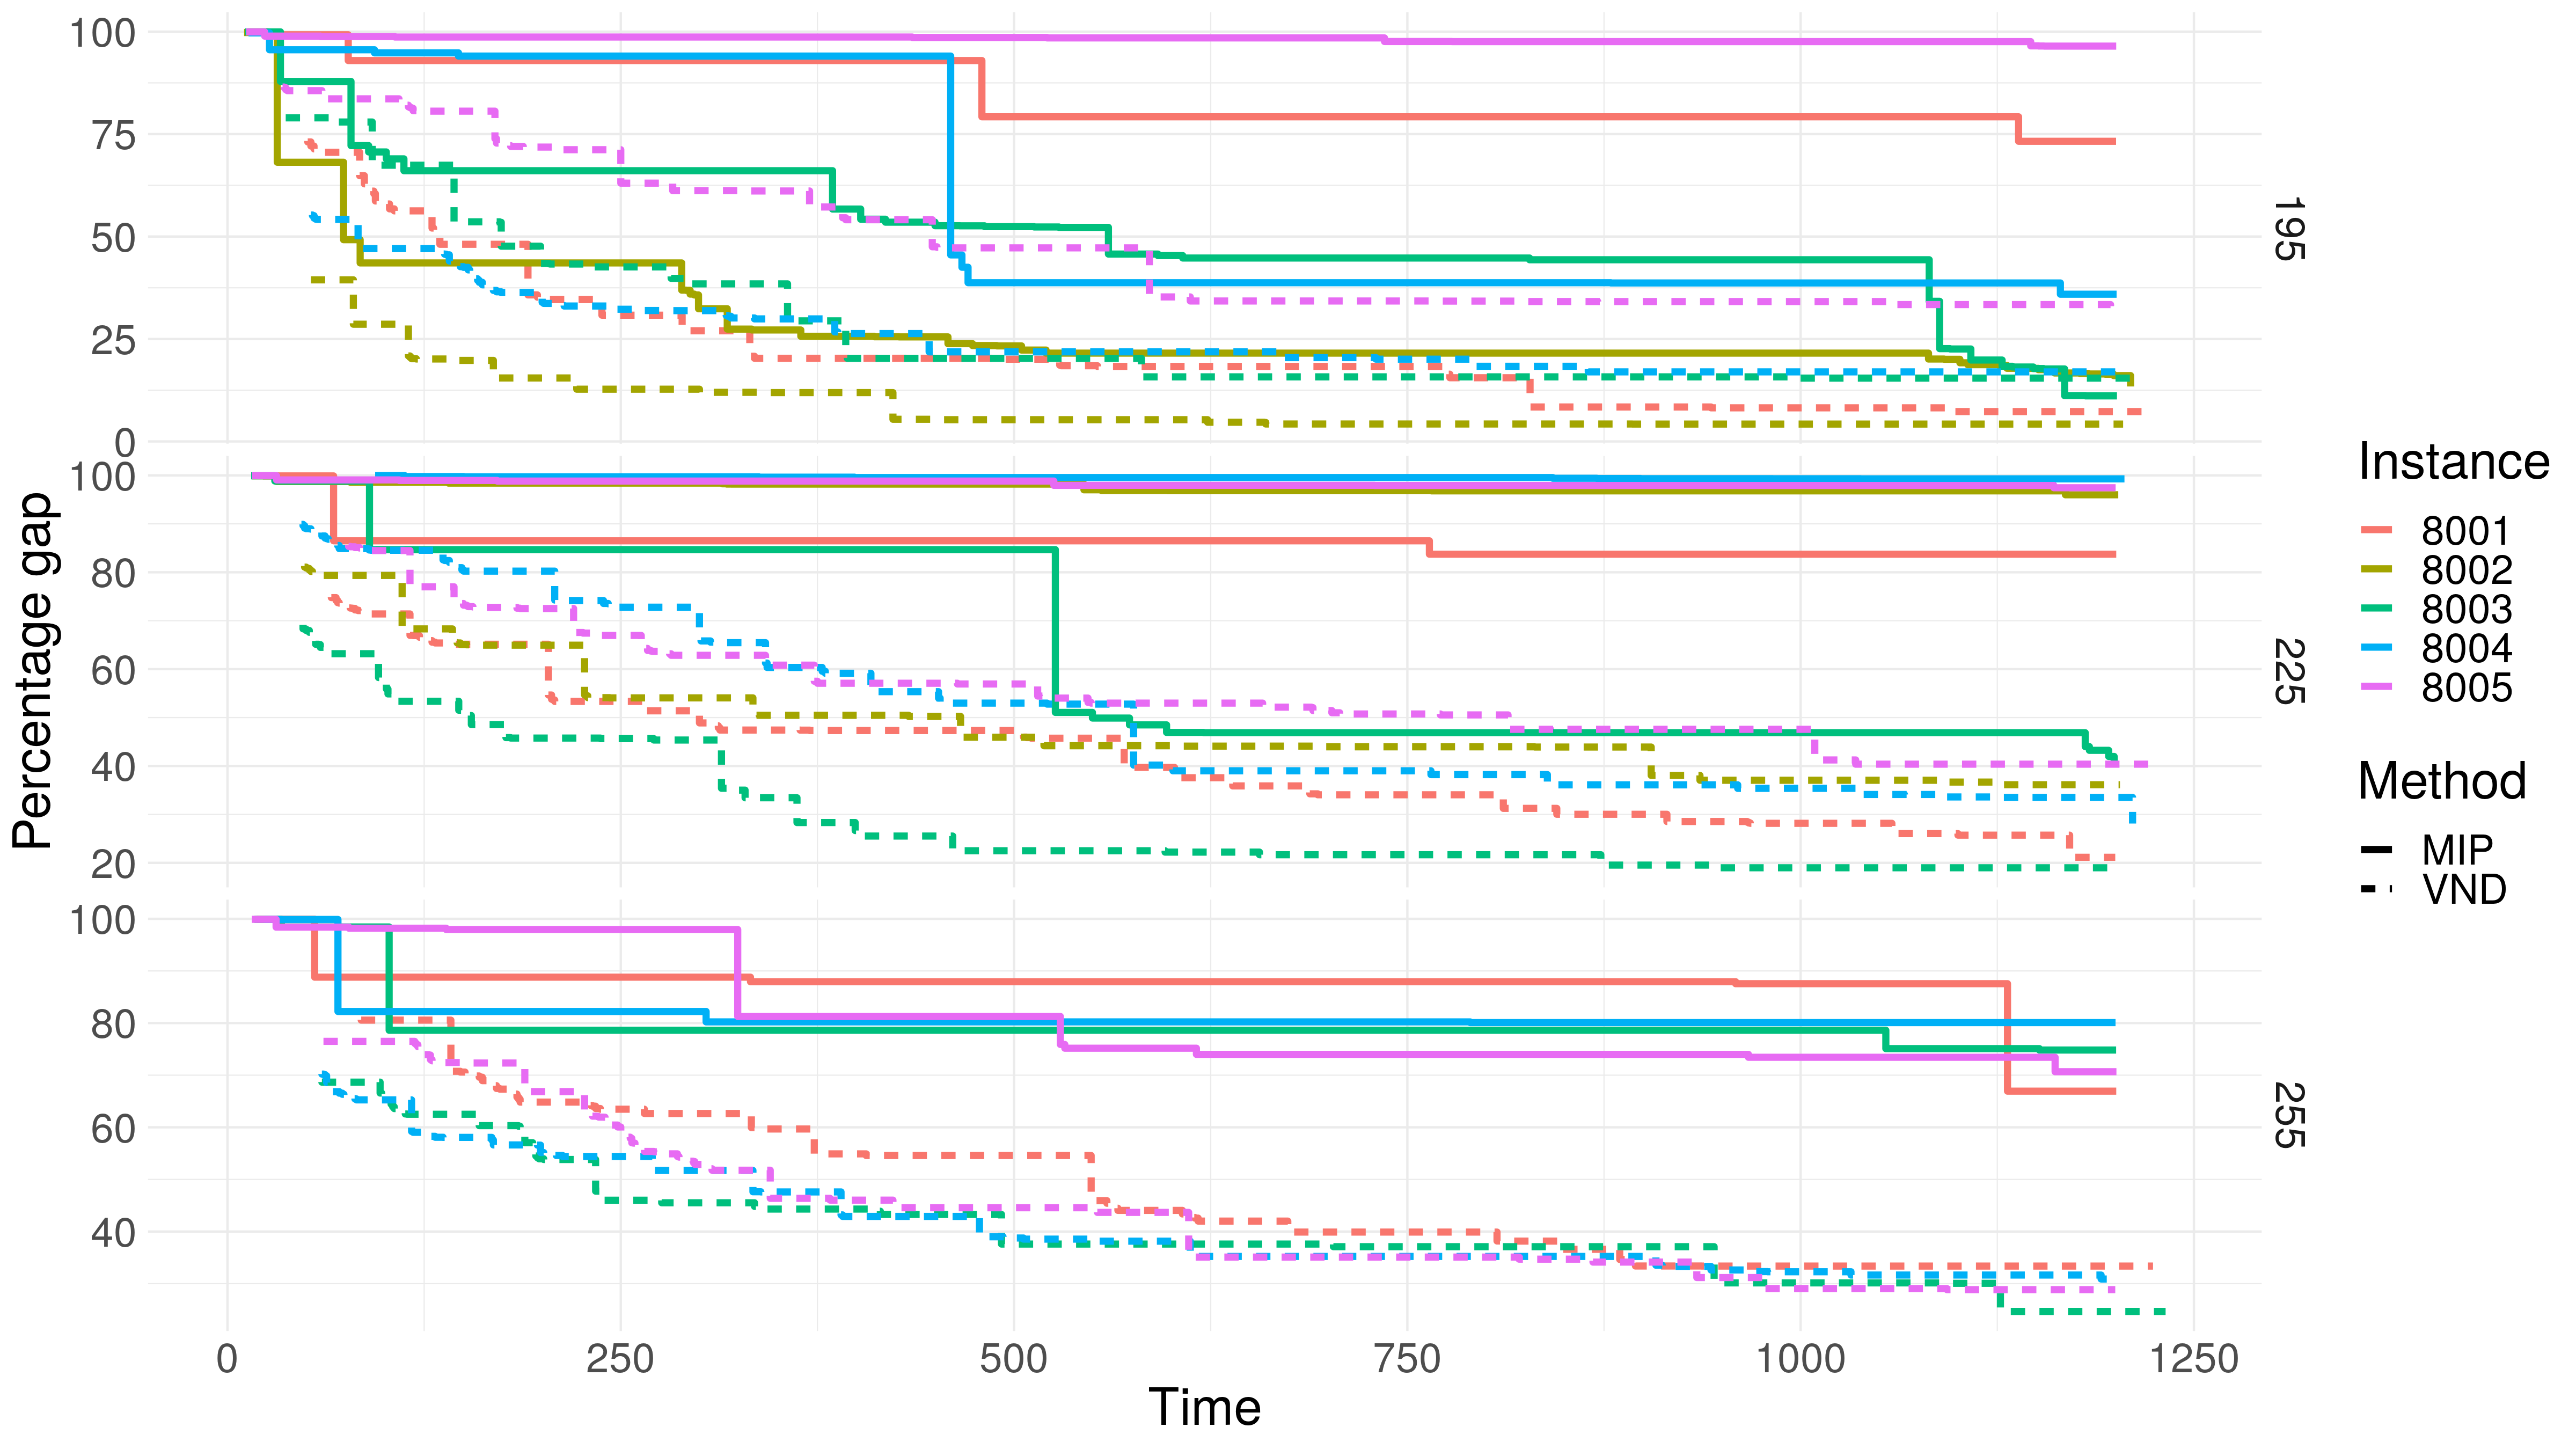
\includegraphics[width=\linewidth]{images/progress_gaps_very_large_255.png}  
  \end{block}{}
\end{frame}

\begin{frame}[t]
\frametitle{\textbf{Preliminary conclusions}}
  % TODO: check phrases
  \pause
  % \begin{block}{}
    \begin{itemize}[<+->]
    \item \textbf{A Graph representation is built} 
      to efficiently explore the solution space of an aircraft and solve the MFMP.
    \item \textbf{Complementary neighborhoods} 
      are combined to avoid falling quickly into local minima.
    \item \textbf{Efficiently solve large instances} 
      by reducing gaps in very large instances from 67.1\% to 23.1\%.
    \end{itemize}
  % \end{block}  
  % \pause
  % \begin{block}{\textbf{Perspectives}}
  %   \begin{itemize}
  %     \item \textbf{Combine with pattern sampling}
  %       e.g., by extracting promising patterns and running a set-covering model as neighborhood.
  %     \item \textbf{Apply graph in GRASP}$\star$
  %       by sampling paths in graph to quickly build solutions.
  %   \end{itemize}
  % \end{block}  
  \pause
  \textbf{To be submitted:} Franco Peschiera, Alain Haït, Nicolas Dupin, Olga Battaïa. Novel Graph-based matheuristic to solve the Flight and Maintenance Planning problem.
\end{frame}

